
\documentclass[fleqn,12pt]{SelfArx} % Document font size and equations flushed left

\usepackage[english]{babel} % Specify a different language here - english by default

\usepackage{lipsum} % Required to insert dummy text. To be removed otherwise
\usepackage{float}
\usepackage{indentfirst}
\setlength{\parindent}{0.7cm}

%----------------------------------------------------------------------------------------
%	COLUMNS
%----------------------------------------------------------------------------------------

\setlength{\columnsep}{0.55cm} % Distance between the two columns of text
\setlength{\fboxrule}{0.75pt} % Width of the border around the abstract

%----------------------------------------------------------------------------------------
%	COLORS
%----------------------------------------------------------------------------------------

\definecolor{color1}{RGB}{94,192,150} % Color of the article title and sections
\definecolor{color2}{RGB}{165,217,190} % Color of the boxes behind the abstract and headings

%----------------------------------------------------------------------------------------
%	HYPERLINKS
%----------------------------------------------------------------------------------------

\usepackage{hyperref} % Required for hyperlinks
\hypersetup{hidelinks,colorlinks,breaklinks=true,urlcolor=color2,citecolor=color1,linkcolor=color1,bookmarksopen=false,pdftitle={Title},pdfauthor={Author}}

%----------------------------------------------------------------------------------------
%	ARTICLE INFORMATION
%----------------------------------------------------------------------------------------

\JournalInfo{Deep Micro Systems, 2018} % Journal information
\Archive{Smart Cities} % Additional notes (e.g. copyright, DOI, review/research article)

\PaperTitle{DeMS White Paper} % Article title

\Authors{Stanley Salvatierra\textsuperscript{1}*, Alvaro Hurtado\textsuperscript{2}} % Authors
\affiliation{\textsuperscript{1}\textit{Chief Technology Officer, DeMS, Smart Cities}} % Author affiliation
\affiliation{\textsuperscript{2}\textit{Chief Executive Officer, DeMS, Smart Cities}} % Author affiliation
\affiliation{*\textbf{Stanley Salvatierra}: s.salvatierra@deepmicrosystems.com} % Corresponding author

\Keywords{Computer Vision --- Smart Cities --- Offline computing --- Artificial Intelligence} % Keywords - if you don't want any simply remove all the text between the curly brackets
\newcommand{\keywordname}{Keywords} % Defines the keywords heading name

%----------------------------------------------------------------------------------------
%	ABSTRACT
%----------------------------------------------------------------------------------------

\Abstract{Privacy concerns and the high demand of GPU capabilities are some of the main problems when dealing with real time video processing, security and safety in the industry and growing cities are some of areas of great demand for such techniques. The rising power of small computers and the increasing availability and effectivity in machine learning techniques allow to design devices capable of detecting events in real time without the need of internet connectivity and a cloud computing service, saving money and solving the increasing privacy problem for business and government. In Deep Micro Systems we achieved to combine several techniques to detect events in real time video and combine the information of several cameras connected to a single device to achieve a good frame rate and a good resolution to capture enough detail in the pictures.}

%----------------------------------------------------------------------------------------

\begin{document}

\flushbottom % Makes all text pages the same height

\maketitle % Print the title and abstract box

\tableofcontents % Print the contents section

\thispagestyle{empty} % Removes page numbering from the first page

%----------------------------------------------------------------------------------------
%	ARTICLE CONTENTS
%----------------------------------------------------------------------------------------

\section*{Introduction} % The \section*{} command stops section numbering

\addcontentsline{toc}{section}{Introduction} % Adds this section to the table of contents

Privacy concerns, low internet conectivity and low computational power are some of the main reasons to improve real time video analisys to work in local devices. The need of internet connectivity or a GPU service are some huge problems that industries and developing countries have to face, increasing costs and not been accesible all the time.

Computer vision has proved to be of great help for industries and governments aimed to increase security and safety at competitive prices, embedded systems have limited power, thus, the need of new computer vision techniques and new hardware for them to handle complex tasks.

Some specific tasks can offer some facilities to real time video monitoring. That is the case of fixed cameras, surveillance cameras and security cameras that can handle only the changind pixels of video to reduce complexity or can make use of computer vision techniques to stabilice the frames in case of a sudden shake of the camera.

Simple computer vision techniques require low computational power and allow the devide to focus machine learning techniques, more heavy, on the main core of the problem to be solved. New, more powerful, small computers are also rising such as Orange Pi, Raspberry Pi 3 B + and even neural sticks like Intel movidius, capable of handling new machine learning techniques.

%------------------------------------------------
\section{Deep Micro Systems}

Deep Micro Systems is a Bolivian Start up in the field of Computer Vision and Smart cities with the mission to  expand the awareness and knowledge industry and governments to smart cities, providing security, efficiency and generating solutions to critical problems in a measurable and sustainable way.

\paragraph{Road Insecurity} The high numbers in roads accidents is currenlty a great concern for Bolivian government with 1300 deaths every year, new technologies are needed in order to reduce this huge numbers and help solve the main problem. As Internet connectivity in Bolivia is expensive and low efficient compared to our neighbor countries, the need of offline processing is a major concern. In order to achieve this Deep Micro Systems designed an All-In-One Device capable of detecting traffic Infringements, generate a visual proof of them and generate valuable real time data for city planning.

In order to generate security in roads and streets, our camera is capable of detecting events in real time video, measure and identify if necessary the vehicle violating law.

\paragraph{Applications of computer vision} Besides road infringement detection, Deep Micro Systems works with computer vision, and it's variety of applications in industry and government. Some of other projects for Deep Micro Systems in the short term are:

\begin{itemize}[noitemsep] % [noitemsep] removes whitespace between the items for a compact look
\item Optimal city design, parking, roads and flows
\item Traffic accidents forecast
\item Smart traffic light managing
\end{itemize}

\paragraph{Industry} Boliviann local business such as Enalbo and IBCO SRL, let us know their interest in detecting real time events such as security infringements of their personal, abnormal functioning of equipment and other failures.

\subsection{All-In-One devices}

The lowering costs of pocket computers and the increasing power and efficiency of machine learning techniques allow to build small devices capable of solve huge problems in cities and in the industry without the need of internet connectivity, guaranteeing privacy and cheaper uninterrupted work.

Computer processors such as Cortex-A53 (ARMv8) 64-bit SoC with 1.4GHz and ARM H3 Quad-core Cortex-A7 with 1.6GHz are capable to handle complex tasks and can make use of the new neural chips to get even faster results in real time.

All this components allow to build custom devices for solving specific problems, providing ethernet connectivity, GPS, GSM/GPRS, Bluetooth, WiFi and any kind of sensors to be required.

\begin{figure}[t]\centering
	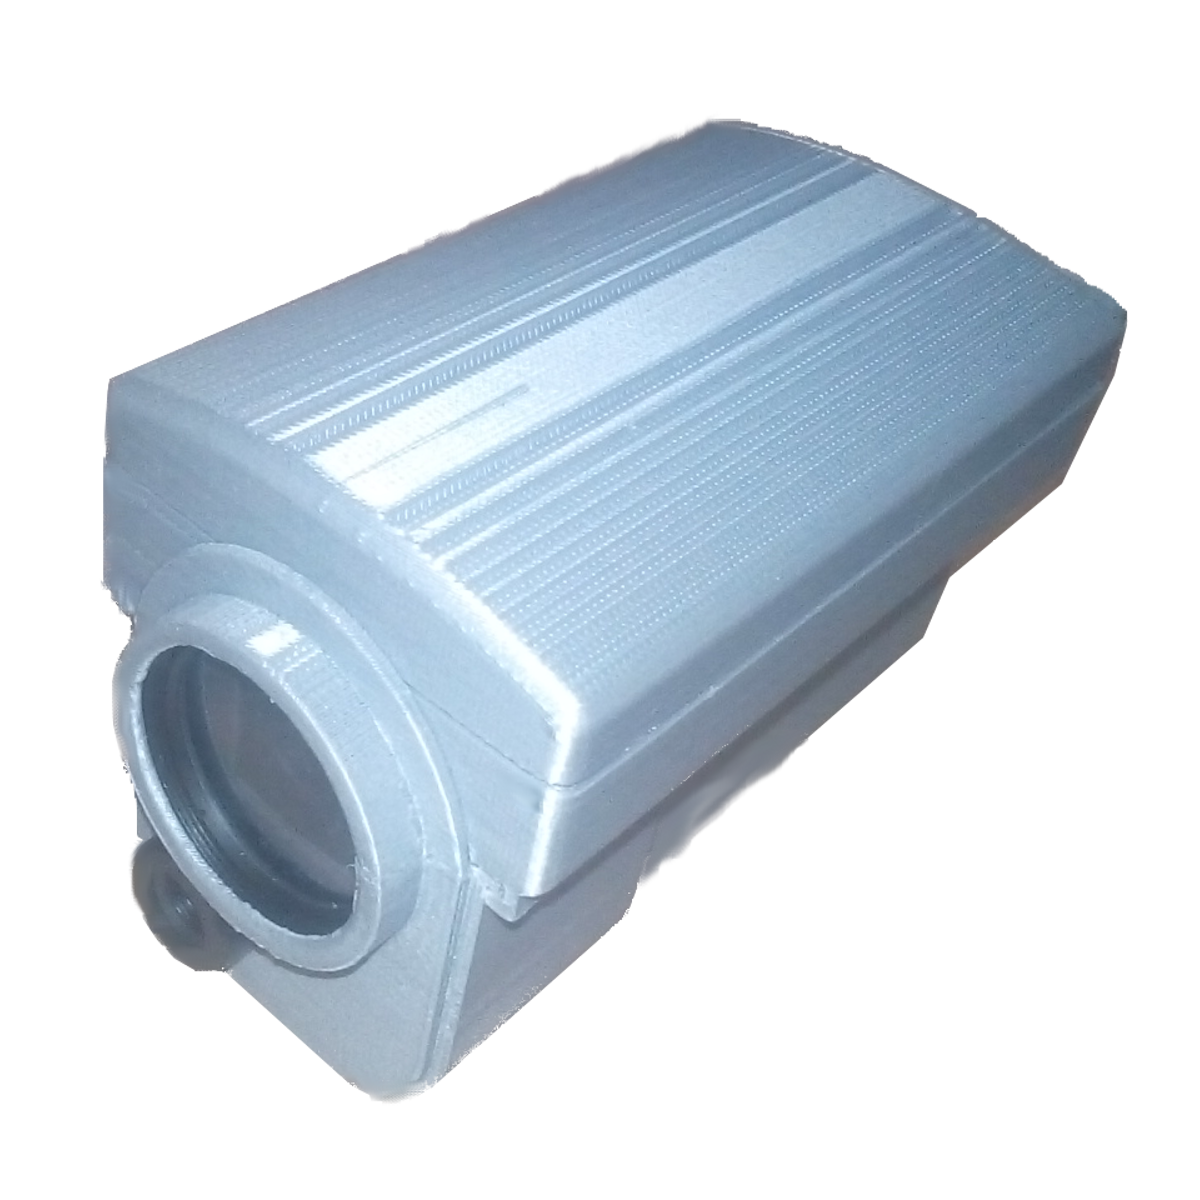
\includegraphics[width=0.8\linewidth]{images/lucam_005}
	\caption{All-In-One computer vision device}
	\label{fig:device}
\end{figure}

Currently Lu-Cam, our smart traffic enforcement camera is a 8x9x16 cm device capable, as seen in figure \ref{fig:device}, and it is capable of detecting events in real time video. Rather than getting frame features with convolutional neural networks, that would take several seconds to complete, we make use of some advantages of their main purpose, extracting only relevant features and making an improvement to less of a tenth of the time it would require. Other techniques continue to appear such as \cite{Cavigelli:2017:CCI:3131885.3131906}, in order to improve efficiency without missing the main objectives of a project.

%------------------------------------------------
\subsection{Real time monitoring and data analysis}

Such All-In-One Devices holds a huge advantage, allowing to pre process data. For example for real time road monitoring we could get real time histograms of infringements and label them according to our needs as shown in figure \ref{fig:histogram}. Then a central computer can handle data from several devices to make desitions, improving efficiency or automating complex process.

\begin{figure}[t]\centering
	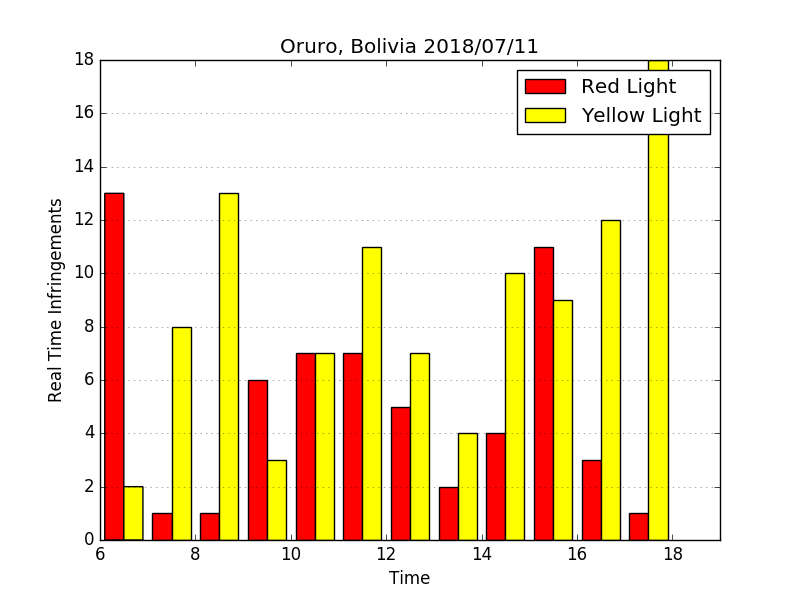
\includegraphics[width=\linewidth]{images/histogram}
	\caption{Real time histogram}
	\label{fig:histogram}
\end{figure}

\begin{figure*}[ht]\centering % Using \begin{figure*} makes the figure take up the entire width of the page
	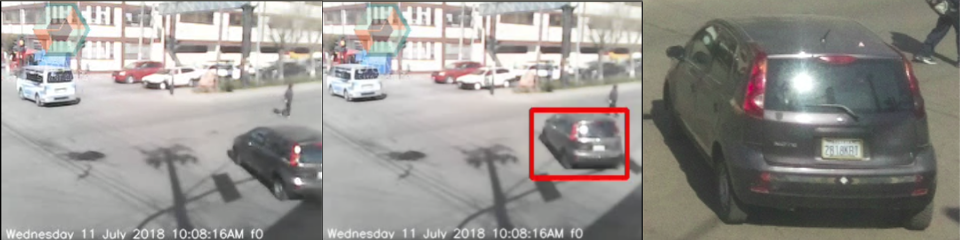
\includegraphics[width=\linewidth]{images/sync}
	\caption{Time synchronization between cameras}
	\label{fig:sync}
\end{figure*}

%------------------------------------------------
\section{On the Edge Computing}

Conventional visual monitoring systems, CCTV, IP cameras, send video transmission, analog or digital, to a data center to be stored and eventually processed or reviewed. Embedded smart cameras process image data directly on-site allowing several advantages over the last systems, in this paper we present:

\begin{itemize}[noitemsep] % [noitemsep] removes whitespace between the items for a compact look
\item \textit{Our approach} to an on-board smart camera computing device.
\item \textit{Hardware and Software description}.
\item \textit{Actual real Use Case implementation} of our product. 
\end{itemize}


Nevertheless, there is a strong demand for mobile vision solutions ranging from object recognition to advanced human-machine interfaces.

\subsection{Our Approach}

The problem of on-board computing and further analysis of real time video is subject of current research. We follow the next procedure which is focused on 3 main cycles that are plot in figure \ref{fig:cycle} and are stated as follows:

\begin{figure}[h]\centering
	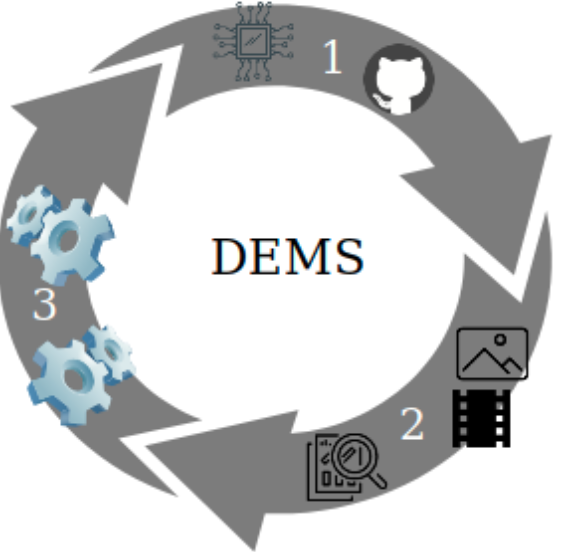
\includegraphics[width=0.7\linewidth]{images/cycle}
	\caption{Cycle of work}
	\label{fig:cicle}
\end{figure}

% Explain the DEMS cicle for target project
\begin{itemize}

\item[1] \textit{Algorithm Design}. If the client requirements does not have precedents, we partially hand craft a Computer Vision Algorithm specific for our client use case for data mining, cleaning and analysis.
\item[2] Data Analysis for client use cases and results presentation according to initial requirements.
\item[3] \textit{Improvement}. Improve original algorithm using the proprietary collected data with the use of Machine Learning techniques, together with a hardware upgrade if required.
     
\end{itemize}

We dedicate a specialized team to solve the problems in each cycle. The case study that we present in the whole proposal, completed 2 of the 3 states of our cycle of work, and we are currently working on an improvement of our main hardware and algorithm to provide the best results to our clients. The collected data is a huge advantage above other competitors and allows us to improve existing products and create new ones.

\subsection{Hardware and Software description}
Below there is a description of the hardware and software we use.

\subsubsection{Software Description}
If the requirements are very specific and no historic data is available, we design an algorithm with traditional computer vision techniques according to the use case with focus on the embedded hardware; we maintain a constant monitoring of the program for the event that client is looking for and at the same time we collect data for three main purposes: Improve the current algorithm with Machine Learning techniques; Bring data for further applications; Create new useful labeled data in the field of work.

Our main tools for the creation of custom algorithms are Python and C++ as main languages. Open-CV is our compendium of multiple purpose Computer Vision techniques which are used to hand craft the desired behavior of the program and data recollection.

\subsubsection{Hardware Description}

The figure \ref{fig:hardware_dec} shows some main aspects of our smart-camera and contains:
\begin{itemize}
	\item A low resolution camera, used to detect flow in real time.
	\item A 8 MP camera sensor is used for capture the main aspects of interest when the low resolution camera triggers the signal of event of interest, in real time.
	\item We also develop custom printed circuit boards to handle different sensors or actuators like the infra-red filter switch for night vision improvements. Custom boards can include several sensors or actuators like GPS, GSM and others 
\end{itemize} 

\begin{figure}[b]\centering
	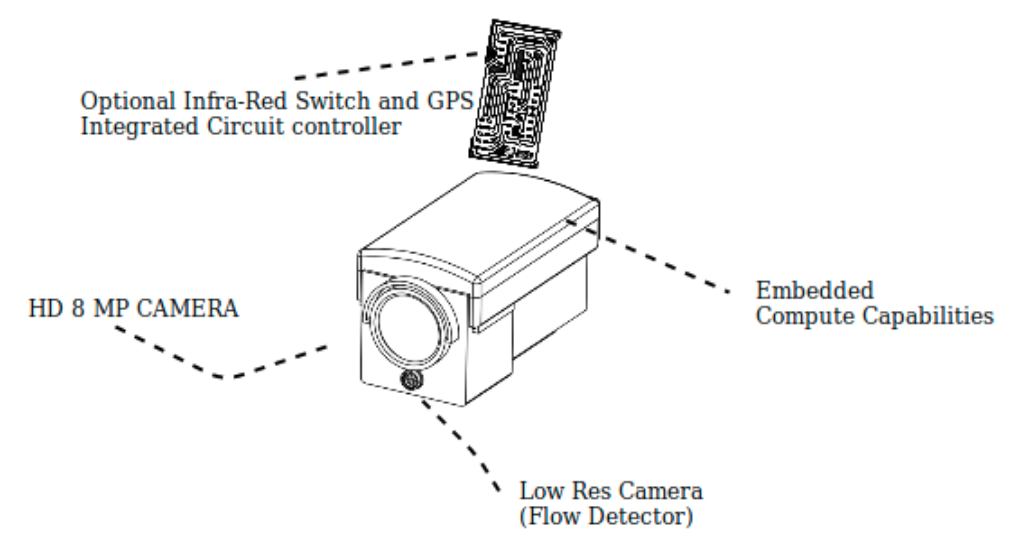
\includegraphics[width=\linewidth]{images/hardware_desc}
	\caption{Hardware schematics}
	\label{fig:hardware_dec}
\end{figure}

The compute capabilities of our embedded device are described below:

\begin{itemize}[noitemsep]

\item SoC: Broadcom BCM2837B0 quad-core A53 (ARMv8) 64-bit @ 1.4GHz
\item GPU: Broadcom Videocore-IV 256 MB VRAM
\item RAM: 1GB LPDDR2 SDRAM
\item Networking: Gigabit Ethernet.
\item 802.11b/g/n/ac Wi-Fi
\item Bluetooth: Bluetooth 4.2, Bluetooth Low Energy (BLE)
\item Storage: Micro-SD
\item Multiple GPIO header
\item Ports: HDMI, analogue audio-video jack, USB 2.0, Ethernet
\item Camera Serial Interface (CSI), Display Serial Interface (DSI)
\item Optional - Neural Network Compute Capabilities according to use case.
\end{itemize}


\subsection{Actual real Use Case implementation}

In figure \ref{fig:work_dec} we present an implementation schematics of our camera.

\begin{figure}[t]\centering
	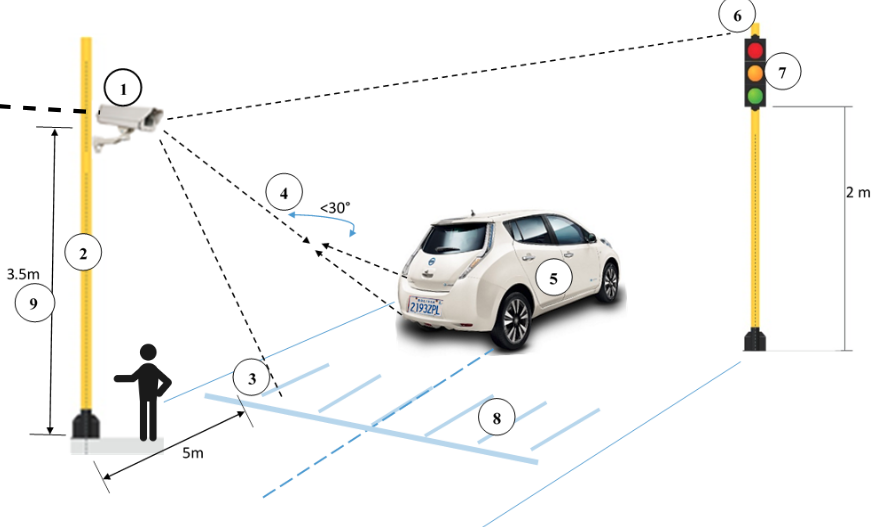
\includegraphics[width=\linewidth]{images/lucam}
	\caption{Actual use case of our embedded camera}
	\label{fig:work_dec}
\end{figure}

\begin{itemize}[noitemsep] % [noitemsep] removes whitespace between the items for a

\item[1]- On Board Computation according to client requirements, communication to a private cloud can be achieved if required.
\item[2]- Mounting pole, in some applications the height of the device plays an important role in the algorithm behavior.
\item[3-8]- Specific working environment, in this case for traffic infringements detection.
\item[4]- Optimal vision angle for plate detection.
\item[5]- Target object, in this case, cars.
\item[6]- Traffic light mounting pole,
\item[7]- Traffic Light signal. The camera is capable of detecting color change if the traffic light is within it's range of optimal working, it is implemented by software but can be implemented as hardware if the client requires.
\end{itemize}
Figure \ref{fig:sync} shows the extract of 5 seconds video from low resolution camera and a picture of High Resolution for target object with region of interest, this two assets, video and picture is the output of our custom algorithm in real time.

As stated before, if an Internet connection is available, we can make a wingspan of the information of video/picture in real time and serve it to different users as required, or save it in a server for further analysis, figure \ref{fig:online} shows the camera and system online behavior.


\begin{figure}[t]\centering
	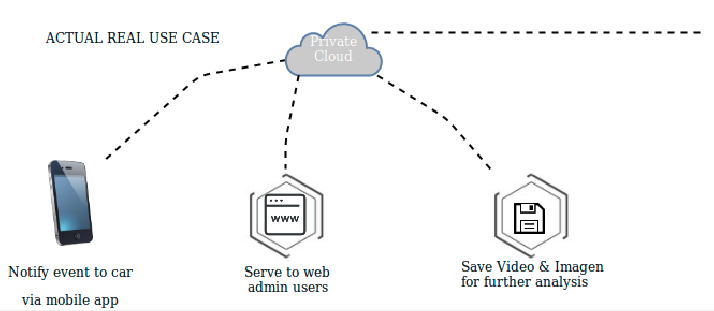
\includegraphics[width=\linewidth]{images/online}
	\caption{On-line process for the information detected in the road. }
	\label{fig:online}
\end{figure}

Currently we are training a Neural Network Algorithm to support the Hand Crafted algorithm with the information of video and image generated from the beginning of this year 2018. Following our cycle of work of Figure \ref{fig:work_dec}, we have generated enough labeled data for our use case and we are ready to start a new cycle of production.

You can see the partial results of this project in our page \href{www.demsbo.com}{www.demsbo.com} and our Github project \href{https://github.com/alvarohurtadobo/prototipo}{https://github.com/alvarohurtadobo/prototipo}.



\section{Further applications}

\begin{figure}[h]\centering % Using \begin{figure*} makes the figure take up the entire width of the page
	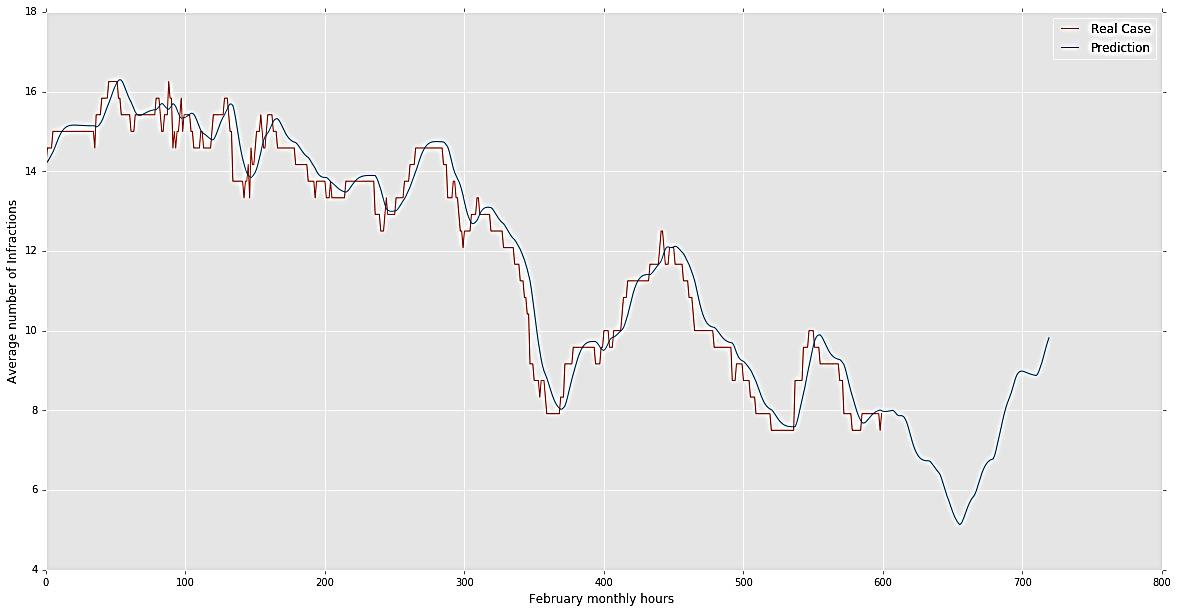
\includegraphics[width=\linewidth]{images/data}
	\caption{Real time Traffic Forecast}
	\label{fig:forecast}
\end{figure}
 
The applications for this kind of devices are endless. Real time monitoring and data analysis can lead us to a better understanding of cause problems and possible solutions to them thanks to data science and big data techniques.

Forecasting data is another example of an application of monitoring systems, in the case of real time traffic monitoring it cann lead to traffic forecasting, saving thousands in time, fuel and possible accidents happening in streets and roads across Bolivia and the world, forecast is possible with a little amount of devices like shown in figure \ref{fig:forecast}



Real time simulation is also possible thank to the real time and flow data in the devices, allowing us to extrapolate data to points where it is not possible to place a monitoring device. Like agressive environments in industries to complex roads in cities.

%------------------------------------------------
\phantomsection
\section*{Acknowledgments} % The \section*{} command stops section numbering

\addcontentsline{toc}{section}{Acknowledgments} % Adds this section to the table of contents

We would like to thank the Unidad de Fortalecimiento Empresarial, El Alto, Unidad de tráfico y vialidad, Oruro and to the Unidad de Tránsito Oruro for the feedback and facilities provided.

%----------------------------------------------------------------------------------------
%	REFERENCE LIST
%----------------------------------------------------------------------------------------
\phantomsection
\bibliographystyle{unsrt}
\bibliography{sample}

%----------------------------------------------------------------------------------------

\end{document}